\documentclass{Mayth}
\begin{document}
\maketitle
\tableofcontents
\chapter*{初高衔接}
\section{高中数学第一课}
\begin{center}
	原文来源:\citet{JiangGaoZhongShuXueDiYiKeDeJiaoXueGouXiang2016}
\end{center}

俗话说,好的开头是成功的一半.进入高中后,学生对每门课的第一节课都充满了期待.高中数学起始课应避免一上来就讲新课内容,可设计成“导游课”,像导游一样,每到一个景点时,先给游客对景点的特色、亮点、注意事项等作一个全貌的介绍.建议高中数学第一课可从两个方面进行构想:\textbf{一方面通过一些实例介绍高中数学之美妙,强调高中数学之重要,对初、高中数学特点进行比较;另一方面介绍高中数学的学习方法}.

\subsection{例说高中数学之美妙}
兴趣是最好的老师!要让学生喜欢数学,最有效的动力就是要激发学生学习数学的热情,让学生的内心能真正感受到数学之魅力,对高中数学充满渴望与期待!
\begin{example}[等势集合]
	请问:长度为1cm的线段上的点的个数与长度为2cm的线段上的点的个数哪个多?

	一部分学生认为2cm的线段上的点的个数多,并且是2倍关系,因为2cm线段的长是1cm线段长的2倍.但也有一部分学生会认为答案是一样多,因为都有无限个,无限就是一样的.

	后面一部分学生回答的答案是正确的,但理由是错误的,因为无限多不一定是一样多.这里可给学生介绍两个无限多元素是相等的需要两者能建立一一对应关系,这一点学生是容易接受的.可从学生与学号开始入手.再通过下图,即可明白.
	\begin{center}
		\tikzset{every picture/.style={line width=0.75pt}} %set default line width to 0.75pt        

		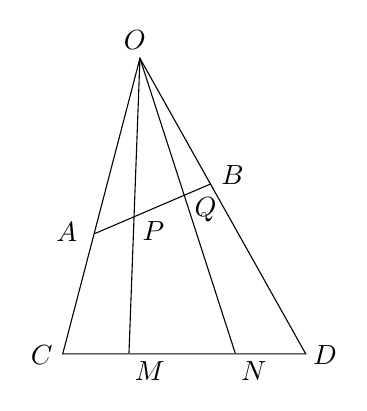
\begin{tikzpicture}[x=0.75pt,y=0.75pt,yscale=-1,xscale=1,scale=0.8]
			%uncomment if require: \path (0,300); %set diagram left start at 0, and has height of 300

			%Shape: Triangle [id:dp8404205470797059] 
			\draw   (322.17,54.17) -- (422,232.17) -- (275.67,232.17) -- cycle ;
			%Straight Lines [id:da9008684259134017] 
			\draw    (294.89,159.78) -- (364.89,129.78) ;
			%Straight Lines [id:da7092672100334034] 
			\draw    (322.17,54.17) -- (315.56,231.78) ;
			%Straight Lines [id:da3275050790851046] 
			\draw    (322.17,54.17) -- (379.56,231.78) ;

			% Text Node
			\draw (310.89,36.07) node [anchor=north west][inner sep=0.75pt]    {$O$};
			% Text Node
			\draw (270.22,151.73) node [anchor=north west][inner sep=0.75pt]    {$A$};
			% Text Node
			\draw (369.56,117.07) node [anchor=north west][inner sep=0.75pt]    {$B$};
			% Text Node
			\draw (254.89,225.73) node [anchor=north west][inner sep=0.75pt]    {$C$};
			% Text Node
			\draw (424.89,225.73) node [anchor=north west][inner sep=0.75pt]    {$D$};
			% Text Node
			\draw (317.56,235.18) node [anchor=north west][inner sep=0.75pt]    {$M$};
			% Text Node
			\draw (381.56,235.18) node [anchor=north west][inner sep=0.75pt]    {$N$};
			% Text Node
			\draw (322.22,151.07) node [anchor=north west][inner sep=0.75pt]    {$P$};
			% Text Node
			\draw (353.56,136.4) node [anchor=north west][inner sep=0.75pt]    {$Q$};


		\end{tikzpicture}
	\end{center}

	紧接着可问:

	(1)长度为1cm的线段上的点的个数与长度为100m的线段上的点的个数哪个多?

	(2)半径为1的圆周上点的个数与半径为2的圆周上点的个数哪个多?

	(3)正整数的个数与正偶数的个数一样多吗?

	(4)有理数与整数的个数一样多吗?

	(5)有理数与无理数的个数一样多吗?

	要告诉学生有理数与无理数是不一样多的,等到大学才能明白,这也是否定“无限多就是一样多的”的一个反例.
\end{example}
\begin{purpose}
	该例是高中第一章集合内容的拓展,通过该例让学生感悟到有限与无限之间有质的区别,在数学中部分可以等于整体,这在日常的生活中是不可思议的,因此本例是激发学生好奇心的很好素材.此外,希尔伯特旅馆的故事都可结合讲.
\end{purpose}
\begin{note}[希尔伯特旅馆\cite{XiErBoTeLuGuanBeiLun2023}]
	假设有一个拥有可数无限多个房间的旅馆,且所有的房间均已客满。或许有人会认为此时这一旅馆将无法再接纳新的客人(如同有限个房间的情况),但事实上并非如此。

	有限个新客人:设想此时有一个客人想要入住该旅馆。由于旅馆拥有无穷个房间,因而我们可以将原先在1号房间原有的客人安置到2号房间、2号房间原有的客人安置到3号房间,以此类推,这样就空出了1号房间留给新的客人。重复这一过程,我们就能够使任意有限个客人入住到旅馆内。

	无限个新客人:另外,我们还能使可数无限个新客人住到旅馆中:将1号房间原有的客人安置到2号房间、2号房间原有的客人安置到4号房间、n号房间原有的客人安置到2n号房间,这样所有的奇数房间就都能够空出来以容纳新的客人。
\end{note}

\begin{example}[杨辉三角]
	通过观察$(a+b),(a+b)^2,(a+b)^3,\ldots$ 展开式的各项系数,介绍杨辉三角.再尝试对 $(a+b)^5$ 的展开.
	\begin{equation*}
		\begin{array}{cccccccccc}
			  &   &   &   & 1      &   &   &   &   & \\
			  &   &   & 1 &        & 1 &   &   &   & \\
			  &   & 1 &   & 2      &   & 1 &   &   & \\
			  & 1 &   & 3 &        & 3 &   & 1 &   & \\
			1 &   & 4 &   & 6      &   & 4 &   & 1 & \\
			  &   &   &   & \cdots &   &   &   &   &
		\end{array}
	\end{equation*}
	本例是高中二项式定理中将介绍的杨辉三角(如图).杨辉三角又称贾宪三角形,帕斯卡三角形,是二项式系数在三角形中的一种几何排列.在欧洲,这个表叫做帕斯卡三角形.帕斯卡(1623—1662)是在1654年发现这一规律的,比杨辉要迟393年,比贾宪迟600年.
\end{example}
\begin{purpose}
	除展示数学结构美之外,渗透归纳思想,同时又渗透一下数学文化.
\end{purpose}

\begin{example}[极限雏形]
	当 $n \rightarrow \infty$ 时, $1+\frac{1}{2}+\frac{1}{3}+$ $\cdots+\frac{1}{n}$ 的值会不会超过 10?超过 100?超过 1 亿?

	有学生会认为超过 1 亿, 他相信积少成多的道理. 老师在肯定答案之时又马上给出变式: 当 $n \rightarrow \infty$时, $1+\frac{1}{2^2}+\frac{1}{3^2}+\cdots+\frac{1}{n^2}$ 的值会不会超过 10?超过 100? 超过 1 亿? 变化之后,连 2 都不会超过. 通过这种相似问题, 但结果又大相径庭, 从而引起学生的认知冲突, 从而激发学生对数学的探究欲望, 告诉学生,这些道理等以后学了极限就清楚了.
\end{example}
\begin{purpose}
	一让学生感受数列的收敛性和发散性, 二让学生再一次体会数学的奇异美.
\end{purpose}

\begin{example}[几何级数]
	电影《漂流瓶》中有一个故事,在船上有几位漂亮的女大学生,同时也有几位文化程度不高的男青年.在这些男青年中有一位绰号叫“三万”的,因为他有三兄弟,父母亲留给他们的财产共10万,平分后每人三万多点,故号称三万.其中一位女大学生想考考“三万”的才华,她说:“我跟你谈恋爱,有个条件:第1天给我1分钱,第2天给2分钱,第3天给4分钱,以后每天给的钱都是上一天的2倍.这样连续给一个月,如果给得起,我就同意.”而号称三万的青年认为这是毛毛雨,说可以,却不知道这是一个圈套.当用计算器按到第10天时,总共需要的钱只有10元2角4分,当按到第20天时,还行,1万多一点,而接下去就很快了,一个月下来给的钱总共大约需要2150多万.

	因为这个数列是成几何级数增长,增长速度之快是出乎人的常识之外.类似的还有折纸游戏,国王奖励国际象棋发明者的故事等等.
\end{example}
\begin{purpose}
	这个知识涉及到高中等比数列求和知识,另一点让学生明白知识的重要性.
\end{purpose}

\begin{example}[几何直觉]
	有两个三角形,其边长分别为17,25,26与17,25,28,求它们的内切圆半径谁大谁小.

	分析: 由 海 伦 公 式 $r=\sqrt{\frac{1}{p}(p-a)(p-b)(p-c)}, p=\frac{a+b+c}{2}$ 可算得: 以 $17,25,26$ 为边长的三角形的内切圆半径 $r_1=6$, 以 $17,25,28$ 为边长的三角形的内切圆半径 $r_2=6$.

	结果为 $r_1=r_2$, 完全出人意外! 估计百分之九十九的人会认为, 这两个三角形的内切圆半径虽然彼此相差不大, 但总应该有些微小差别, 绝对不会是相等的.
\end{example}
\begin{purpose}
	数学中直觉不一定可靠, 有时需要严密论证.
\end{purpose}

\begin{example}[数学悖论]
	一个理发师给自己立了这么一条店规:“只给那些不给自己刮脸的人刮脸.”那么,这位理发师的脸该不该由他自己刮?

	如果理发师的脸由他自己刮,则他属于“自己给自己刮脸的人.”因此,理发师不应该给自己刮脸;如果理发师的脸不由他自己刮,则他又属于“自己不给自己刮脸的人.”因此,他的脸可由自己刮,这显然又与上述“自己不给自己刮脸的人”相矛盾.从以上分析,这样不对,那样也不对,就是数学中的悖论.
\end{example}
\begin{purpose}
	激发学生对数学逻辑的兴趣,同时也可介绍数学发展的几次危机.
\end{purpose}

\subsection{例说高中数学之重要}
做一件事光有兴趣是远远不够的,只有认识到做这件事的意义和重要性,才能有做好这件事不竭的动力,学习数学也是一样.数学学科是一门基础学科,它的重要性是多方面、多角度、多层次的.

1. 数学是一种描述自然的语言.

数学语言刻画事物的数量关系、形式与形状,反映事物的本质属性.当人们需要把客观事物的认识精确化的时候,必须使用数学语言. 诺贝尔物理学奖获得者菲曼曾说:“要是没有数学语言,宇宙几乎是不可描述的!”例如,牛顿用数学公式展示了物质运动的三大定律,爱因斯坦用黎曼有关弯曲空间曲率理论阐述广义相对论;化学家、生物学家、经济学家等都必须用数学语言使自己的学科精密化.

2.数学是培养思维能力的重要载体.

法国数学家格瑞斯曼说过这样的话:“数学除了锻炼敏锐的理解力,发现真理外,它还有另一个训练全面考虑和科学系统的头脑的开发功能.”

通过数学学习,形成一种数学思想和能力,明确数量观念,注意事物的数量关系与变化规律;通过数学学习,了解数学的概念、方法、理论等的产生和发展的渊源及过程,了解和领会从实际出发建立数学模型,再到解决问题的全过程;通过数学学习,提高人的逻辑思维能力,能在纷繁复杂的各项工作面前有条不紊地处理等.

\begin{example}
	甲、乙二人在一圆形桌面上轮流放面值一样的硬币,不可重叠,当谁放不下了,谁就输.如果甲先放,问有无必胜的策略?
\end{example}

\begin{analysis}
	如果甲、乙二人随意去放,显然甲不一定能赢.但如果能从数学对称原理去想,先放者就有必胜的策略.只要甲第一次先放在桌子的中心,接下来乙放,然后甲放在乙刚放的关于圆心的对称点上,依次下去,由对称原理,只要乙能放,甲肯定能放,故甲胜.

	本题将随意放硬币的游戏进行有序化,先夺取“战略高地”,这就是数学的思维.
\end{analysis}

\begin{example}
	证明: 任意6人中,至少有3人两两相互认识或两两互不认识.
\end{example}

\begin{analysis}
	这一问题如果将各种情况都加以考虑,也是一种思路,穷举法,但情况比较多,显得繁杂.现在将问题进行数学化,就不难了.将6人视为平面上6个点,相互认识的用实线相连,相互不认识的用虚线相连.

	先考虑从A点出发与其它五个点连线情况,共有5条线,由于只有实线与虚线二种情形,因此由抽屉原理可以断定这5条线中至少有3条是同一类型的,譬如,有3条实线AB,AC,AE,现在分析B,C,E三点之间的连线,若B,C,E三点之间的连线有一条是实线,譬如BE,那么A,B,E三者的连线都是实线,问题解决,反之,若B,C,E三点之间的连线都是虚线,问题也得证.
\end{analysis}

3.数学是科学技术进步的直接推手

我国著名数学家华罗庚先生曾说:“宇宙之大,粒子之微,火箭之速,化工之巧,地球之变,生物之谜,日用之繁等各个方面,无处不有数学.”由此可见数学应用是非常广泛的.

二十世纪科学技术进步给人类生产和生活带来的巨大变化确实令人赞叹不已.从远古时代起一直是人们幻想的“顺风耳”、“千里眼”、“空中飞行”和“飞向太空”都在这一世纪成为现实.回顾二十世纪的重大科学技术进步,以下几个项目元疑是影响最大的,而数学的预见和推动作用是非常关键.

(1)先有了麦克斯韦方程,人们从数学上论证了电磁波,其后赫兹才有可能做发射电磁波的实验,接着才会有电磁波声光信息传递技术的发展.

(2)爱因斯坦相对论的质能公式首先从数学上论证了原子反应将释放出的巨大能量,预示了原子能时代的来临.随后人们才在技术上实现了这一预见,到了今天,原子能已成为发达国家电力能源的主要组成部分.

(3)牛顿当年已经通过数学计算预见了发射人造天体的可能性,差不多过了将近三个世纪,人们才实现了这一预见.

(4)电子数字计算机的诞生和发展完全是在数学理论的指导下进行的.数学家图灵和冯诺依曼的研究对这一重大科学技术进步起了关键性的推动作用.

(5)遗传与变异现象虽然早就为人们所注意.生产和生活中也曾培养过动植物新品种.遗传的机制却很长时间得不到合理解释,十九世纪60年代,孟德尔以组合数学模型来解释他通过长达8年的实验观察得到的遗传统计资料,从而预见了遗传基因的存在性.多年以后,人们才发现了遗传基因的实际承载体,到了本世纪50年代沃森和克里发现了DNA分子的双螺旋结构.这以后,数学更深刻地进入遗传密码的破译研究.

数学是人类理性思维的重要方式,数学模型,数学研究和数学推断往往能作出先于具体经验的预见.这种预见并非出于幻想而是出于对以数学方式表现出来的自然规律和必然性的认识,随着科学技术的发展,数学、预见的精确性和可检验性日益显示其重意义.

\subsection{高中数学与初中数学的差异}
1. 知识差异

初中: 内容少、浅、面窄,常量为主, 题型少、简单,可反复磨炼,甚至死记硬背就可以考出高分.

高中:知识多、深、面宽;变量为主, 题型多, 没有时间反复.

2. 教法差异

初中: 课堂容量小,讲速慢,题型少,反复,模仿.

高中: 课堂容量大,知识复杂,速度快,题型多,很少反复.

3. 学法差异

初中: 自学能力差, 讲授, 被动学, 反复练.

高中:自主探索, 主动学习, 获得知识的渠道宽.

4.语言差异

初中:初中的数学主要是以形象、通俗的语言方式进行表达.

高中: 高一进来就触及抽象的集合符号语言、逻辑运算语言、函数语言、图形语言等, 也就是说抽象化程度大大提升,抽象是感觉难的主要原因.

5.思维差异

初中:很多老师为学生将各种题型建立了统一的思维模式(如:解分式方程分几步;因式分解先看什么、再看什么,等等),确定了常见的思维套路,因此,形成初中阶段在数学学习中习惯于这种机械的、便于操作的定式.

高中:在解题方法步骤上灵活多变,往往能一题多解,用代数法能解出,用几何法也能解出,但每种解题方法所用时间和出错的机会不一样,这就要求对各种思想方法如数形结合、分类讨论、整体换元、消元等思想方法融会贯通,思想方法的学习就像外语的语法一样,在高中数学的学习中占很大比例.

\subsection{高中数学学习方法}
(一)高中数学的学习方法六字方针:思考,运算,积累.

1.思考是核心.

学数学有时课堂上都能听懂,老师讲的题目觉得自己都会,可是课下自己一做就错,有的问题甚至没有思路.学数学最忌讳的是老师讲同学听,听完之后做笔记,从头听到尾,从头记到尾,听的特明白,笔记记得特清楚,轮到自己一做题还是不会做,还是无处下手,这就好比同学们站在岸上学游泳,没有经过那个被水淹、在水里扑腾的过程,老师示范的再清楚你还是白搭.要将思考贯穿于数学学习的整个过程,无论课上老师的提问,还是课下自己做题,我们始终要做的就是思考:为什么这样做,为什么要这样变形,这道题还能怎么做,这类题目解决的共同方法是什么,所蕴含的思想方法是什么,等等.数学学习的主阵地是课堂,老师提出问题后同学们的大脑就要飞速地旋转,哪怕有一点点思路也要积极回答,这样积极参与的过程学习效率很高.

2.运算是基础.

数学离不开算.在小学阶段被称为算术,初中阶段被称为代数,用字母代替数字进行运算,在高中更是通过指数、对数、三角函数、向量、排列组合、算法等载体发展人的计算能力.较复杂的解析几何题目运算过程可达几十步,只要错了一个正负号或算错一个小数就会满盘皆输,整个大题报废,离开了一个强大的计算能力就谈不上学好数学.所以说,一道题从有了思路到完整解答还差多少里?十万八千里!为了提高计算能力,在笔算的基础上更要心算.学数学要将算放在首位,这也是对数学的第一个也是最重要的一项要求.运算是能力,能力的提升没有什么巧妙的方法,就是要拿出你的耐心和细心大量地练,亲自动手将每一个得数算出来,当然还要掌握好算理.

3.积累是保障.

数学课如果有几节课没听,有几节练习没跟着做,再接着听便不好听懂,甚至一点都不会.由此可见数学的一个重要特点就是必须将先学的知识彻底掌握才能进行后续的学习.前边提到数学的一个重要特点就是抽象,内容都是用字母和符号表达的,这就要求同学们必须对学过的东西进行持之以恒的反复记忆和运算,通过这种方式将抽象的东西内化,最后形成直觉.但数学题太多了,人们都把它比喻成题海,都记不把人累死吗?这就涉及到积累什么东西的问题.牵牛要牵鼻子,想问题办事情要抓关键,抓主要矛盾.高中数学的这个关键就是指好题:有代表性的,通过这道题能掌握好几个重要知识点,能掌握解一类问题的通法,能以一顶十的题目.要是让你单纯背诵你总觉得这事有点荒唐,不像文科的东西那样好背,或者说根本就不适合背诵,怎么办?多做,好题做六遍,做的遍数多自然就掌握了.所以我们要积累的东西是上课老师所讲授的典型例题,解决典型例题的思想方法.课上要逐渐学会迅速记录简明的课堂笔记,课下详细整理,补充详实.除此之外还有学着整理做过的试卷,这些试卷上往往有很多精彩的题目,都往笔记本上誊写没那时间,索性直接将笔记做在卷子上,每隔一段时间进行阅读,尤其是考前这么做效果最好.

(二)五点建议

1.认真听好每一节课

有的同学上课不听,下课不看,资料不做,考试前拿着课本在那记公式,总结知识点,考试成绩是一塌糊涂.原因是什么?为什么初中可以考前突击,现在却不行了?初中知识简单,结构单一,高中数学灵活多变,不是靠死记硬背,更多的是课堂上讲解的解题的思想方法.

2.做好数学笔记

特别是对概念不同侧面的理解,以及典型例题.

3. 建立数学错题本

把平时容易出现错误的知识或推理记载下来,以防再犯.争取做到:找错、析错、改错、防错.达到:能从反面入手深入理解;能由果溯因把错误原因弄个水落石出、以便对症下药;解答问题完整、推理严密.

4. 记忆数学规律和数学小结论

高中数学不是靠死记硬背,但是不代表不背,基本的规律和结论还是必须记的,记的熟练了,自然也就能灵活运用了.

5. 学会总结归类

(1)从数学思想分类;(2)从解题方法归类;(3)从知识应用上分类.

\note{本文从四个方面设计高中数学起始课,由于内容多,建议用两种方式灵活处理,一是上两节课;二是精简内容,并结合教师自己的特长与兴趣进行设计.}

%\chapter{集合与常用逻辑用语}
\section{集合的概念}
\marginnote{2024-7-31}
\subsection{教材分析与教学重难点}
重点: 元素与集合的"属于"关系, 用符号语言刻画集合.

难点: 用描述法表示集合.
\subsection{教学目标}
\begin{enumerate}
	\item 通过示例,了解集合的含义,理解元素与集合的属于关系.
	\item 对于具体问题,能在自然语言和图形语言的基础上,用符号语言表示集合.
	\item 在具体情境中,了解全集与空集的含义.
\end{enumerate}
\subsection{学情分析}

\subsection{教学方法}

\subsection{板书设计}
\begin{boardenv}[集合的概念]
	\begin{enumerate}
		\item 集合的概念\\
		      一般地,我们把研究对象看作是\textbf{元素},把一些元素组成的整体看作是一个\textbf{集合}.
		\item 性质\\
			  确定性、互异性
		\item 属于关系\\
		      $a$属于集合$A$: $a\in A$\\
		      $a$不属于集合$A$: $a\notin A$.
		\item 集合的表示方法\\
		      描述法\\
		      列举法
	\end{enumerate}
\end{boardenv}



\subsection{教学过程}
\begin{intro}[教学片段\cite{HouCongShuXueHaoWanDaoWanHaoShuXueGaoZhongShuXueDiYiKeBuFangCongWan2020}]
	面对新的教师,新的同学,学生往往比较拘谨,不敢表达,这无疑会影响教师教育教学的质量.故而,教师在课程导入时,不妨以集合的“确定性”为背景和学生开一个小玩笑.班长:起立!学生:老师好!教师笑语:同学们好!请所有长头发的同学站一下,其余同学请坐下.(停顿几秒给学生思考)教师继续:(目测包含所有站着的学生)请站着的同学中身高低于2米的坐下.
\end{intro}
\begin{purpose}
	意在建立学生对集合概念的感性认识.“长头发”的不确定性引发学生思考:多长的头发算长头发?部分头发较长的女生不知所措,有的男生也在纠结自己的坐与站的问题.教师快速追加坐下的条件“身高低于2米”,则所有站立的学生坐下,化解了这一部分学生的尴尬.课堂上,师生谈笑间拉近了心理的距离.
\end{purpose}

\begin{intro}
	教师开始本节课的导入语:首先祝贺大家升入高中的学习,老师刚刚以高中数学中“集合”的概念为背景和大家开了一个小玩笑.什么是集合?我们全班的全体同学可以是一个集合,全体的男同学或全体的女同学也都是一个集合,但所有长头发的同学不能构成一个集合,因为集合要满足其内在的个体(元素)是确定的.这也是引发部分同学不确定自己是坐还是站的原因,而站着的同学中“身高低于2米的同学”显然是能够确定的,它是一个集合.集合是现代数学的一个基本概念,也是我们高中数学学习的第一个概念.同学们在后续的学习中要注意数学概念的学习,概念的理解程度决定了我们数学学习的深度,也直接决定了数学解题水平的高低.
\end{intro}
\begin{purpose}
	通过学生不难理解的集合概念,让学生体会数学概念在数学学习中的重要性.教学中,教师不必对集合的概念加以定义,以学生的感性认识理解即可,意在提升学生的学习兴趣和数学认知,也可留下悬念为后续正式学习集合相关知识铺垫情感因素.
\end{purpose}

\subsection{归纳总结与作业布置}
\section{集合的表示方法}
\subsection{教材分析与教学重难点}

\subsection{教学目标}

\subsection{学情分析}

\subsection{板书设计}

\subsection{教学过程}

\subsection{归纳总结与作业布置}

\section{集合的基本运算}
\subsection{教材分析与教学重难点}

\subsection{教学目标}

\subsection{学情分析}

\subsection{板书设计}

\subsection{教学过程}

\subsection{归纳总结与作业布置}

\section{}
%\chapter{一元二次函数、方程和不等式}

%\chapter{函数的概念与性质}
\section{函数的概念}
\newpage
\section{函数的奇偶性}
\subsection{教材分析}
本节课\cite{YuAPOSSiDuanShiJiaoXueSheJiKeTiHanShuDeQiOuXing2024}所用教材为2019年人教A版《普通高中教科书 $\cdot$ 数学》, 选择的教案内容为其中的第 3 章(《函数概念与性质》) 的3.2.2节, 探讨函数奇偶性特征.

本章在开始之初, 首先简单地介绍了函数的基本概念(即函数反映变量关系而构建起的数学模型) , 然后在此基础上探讨了函数的基本性质(单调性) . 在本节中, 重点是探讨函数的奇偶性, 为后续研究幂函数、对数函数等多种函数性质奠定基础, 也能方便后续对相关函数性质的深刻理解.

\subsection{教学目标}
\begin{enumerate}
	\item 指导学生能够通过数量关系来判断出函数图像的对称类型: 是原点对称,  $x$ 轴对称还是 $y$ 轴对称, 然后在此基础上明确奇偶性的相关定义.
	\item 学生能够根据自己掌握的知识, 对函数的奇偶性与否作出判断.
	\item 要求学生能够把握数形结合思想精髓, 能够遵循由特殊到一般(具体到抽象) 的思考和研究过程, 提升个体的思维能力, 深刻感受函数性质的相关研究适用方法.
\end{enumerate}

\subsection{学情分析}
本节课是针对高一学生开展授课, 学生具备的知识、方法和能力特征分别如下:

(1) 具备深入探究的知识基础;

(2) 具备数量关系刻画方法;

(3) 能够从数量关系层面简单地刻画函数对称性, 但对数形转化过程不够清晰. 最终确定了该节课的主要教学内容, 明确了其中的难点和重点内容, 即了解 $f(-x)=$ $f(x)$ (或 $f(-x)=-f(x)$ )的表达意义.

\subsection{教学方法}
本教学设计以 APOS 理论为基础, 根据该理论的 4 个阶段来完成相关教学设计过程.
\begin{enumerate}
	\item 活动阶段: 设置学生自主探究活动, 让学生在实际探究过程中获得对所学知识点及其背景的直观了解, 方便本文后续的函数奇偶性教学的顺利开展.
	\item 过程阶段: 深入思考活动阶段的探究内容, 鼓励学生在头脑中对其进行详细的描述, 将其转化为思维的内化内容, 并对活动中的相关内容进行总结反思, 引导学生能够通过抽象的方法揭示出函数奇偶性的基本特征.
	\item 对象阶段: 经历上述两个阶段以后, 学生对基础性概念的理解日益完善, 能够通过形式化的符号和定义来抽象出函数奇偶性的本质特征.
	\item 图式阶段: 在这一阶段中, 需要引导学生能够在旧的知识基础上, 与新的知识建立起基本联系, 能够将函数奇偶性的相关概念、特征与其他的定理和性质构建起内在脉络, 形成有关结构性的知识导图.
\end{enumerate}

\subsection{教学过程}
\subsubsection{活动阶段}
% 活动1
\begin{activity}
	让学生观察大自然和生活中存在的轴对称与中心对称图形, 然后鼓励学生根据自己的知识经验来列举出在学习或生活中碰见的相关图形, 能够将学生的观察和想象与实际的教学情景衔接, 从而顺利地实现学生的自主探究向相关教学内容的顺利过渡.

	问题 1 : 说出展示的图形分别属于哪种对称图像?

	问题 2 : 你在生活中还能遇到哪些中心或轴对称图形?

	% \includegraphics[max width=\textwidth, center]{2024_10_21_5f8330c8eaf7c7eac80fg-2}

	问题 3 : 数学中哪些函数的图像具有对称性. 问题 4 : 举出具有对称性的函数的解析式.
\end{activity}
% 设计目的
\begin{purpose}
	设计生动有趣的数学问题, 帮助学生在现有的认知基础上, 利用一些推理和判断方法, 寻找到对称性图像的本质特征, 激发学生的学习兴趣和内在动力.
\end{purpose}

% 活动2
\begin{activity}
	引导学生用"形"探究.

	问题 5 : 指出 $y=x^{2}, y=|x|$ 图像具备哪些共同特征?

	问题6:如何证明函数图像是 $y$ 轴对称图像?

	问题7: 图像是由点构成的, 图像关于 $y$ 轴对称, 那么在 $y$ 轴两侧的图像中相应点坐标之间存在什么关系?

	问题8: 通过直尺测量的方式, 告诉我们这两个点在横纵坐标上关系究竟如何?

	问题9: 是否还能够发现其他对称点的对称关系?
\end{activity}
% 设计目的
\begin{purpose}
	让学生对函数图像产生直观感知, 引发学生的独立思考和主动探索, 通过测量或折纸的方式调动学生参与具体教学的积极性, 形成良好的自主探索兴趣, 从而揭示出偶函数性质特征.
\end{purpose}

% 活动3
\begin{activity}
	引导学生用"数"探究.

	问题 10 : 根据计算得到的数值填写完成下表 1 , 并观察数值两者之间的关系.

	表 1 : 函数 $f(x)=x^{2}$

	\begin{center}
		\begin{tabular}{|c|c|c|c|c|c|c|c|c|c|}
			\hline
			$x$ & $\ldots$ & -3 & -2 & -1 & 0 & 1 & 2 & 3 & $\ldots$ \\
			\hline
			$y$ & $\ldots$ & 9  & 4  & 1  & 0 & 1 & 4 & 9 & $\ldots$ \\
			\hline
		\end{tabular}
	\end{center}

	表 2 : 函数 $f(x)=\mathbf{2}-|x|$

	\begin{center}
		\begin{tabular}{|c|c|c|c|c|c|c|c|c|c|}
			\hline
			$x$ & $\ldots$ & -3 & -2 & -1 & 0 & 1 & 2 & 3  & $\ldots$ \\
			\hline
			$y$ & $\ldots$ & -1 & 0  & 1  & 2 & 1 & 0 & -1 & $\ldots$ \\
			\hline
		\end{tabular}
	\end{center}

	问题 11: 关于 $y$ 轴对称的每一组点, 是否都有 $x$ 互为相反数,  $y$ 相等的特征?

	问题 12 : 这两个函数的定义域是什么? 是否存在对称关系?

	问题 13 : 对表 1 和表 2 进行观察, 告诉我们函数图像特征.

	问题 14: 对于任意的 $a \in \mathbf{R}$ ( $a$ 为常数), $f(-a)=f(a)$ 是否存在?

	问题 15: 对于任意 $x$ (定义域内) ,  $f(-x)=f(x)$ 是否存在?

	问题 16: 任意一个关于 $y$ 轴对称的函数图象,  $f(-x)=$ $f(x)$ 是否成立?

	问题 17: 对于定义域内任意一个 $x, f(-x)=f(x)$ 恒成立, 是不是就意味着该函数为 $y$ 轴对称函数?

\end{activity}
% 设计目的
\begin{purpose}
	此次教学设计的主要意图在于帮助学生认识到数学教学不能简单地理解为数学知识教学(即单纯地传播数学知识点) , 而是一种帮助学生养成数学思维, 促进学生发展, 捕捉数学价值的教育方式.

	数学教学的核心在于数学思想的灌输, 包括函数与方程、数形结合、分类讨论、化归与转化、特殊到一般等. 上述设计的 5 个问题, 能够帮助学生逐渐从动眼动手向动脑动心转化, 让学生在探索的过程中总结数学规律, 揣摩数学思想, 掌握由具体到抽象的思维过程.
\end{purpose}


\subsection{过程阶段}
"过程阶段"是对"活动阶段"进行的外显数学活动的进一步思考. 学生通过对上一阶段活动的重复参与, 能够在脑海中形成一系列复杂的数学思想过程, 进行相对深层次的抽象思维归纳和推理分析, 从而把握教学内容的本质特征.

\subsubsection{偶函数定义的引入}
以 $f(x)=x^{2}, f(x)=2-|x|$ 函数为例, 在进行相关定义时, 首先要明确函数定义域, 然后在此基础上来探索两个函数关于原点对称的特征, 同时又发现 $f(-x)=f(x)$ , 于是将其称作为偶函数.

讨论 1 : 结合前文的推导过程开展广泛的小组讨论, 鼓励学生自行归纳出偶函数的定义.
\begin{purpose}
	学生通过前面的思维和探索步骤自主完成了偶函数的定义过程, 是本章节教学内容的核心部分, 同样也是检验前期探索过程的重要途径.
\end{purpose}

\subsubsection{类比联想, 得出奇函数定义}
经过了对偶函数的探究和定义过程, 就是应该放手让学生自主探究奇函数的定义, 鼓励学生通过类比的方法得到相关的准确定义描述.
\begin{purpose}
	教师要充分地信任学生, 敢于放手交给学生自主探索, 而不是想尽方法来限制学生, 影响学生的思维能力的发挥. 学生在进行奇函数定义探索时, 可以完全照搬偶函数的整个探索过程, 然后自主得出相关的函数定义.
\end{purpose}

\subsection{对象阶段}
在这一阶段, 需要将学生探究出的奇偶函数本质特性通过形式化的符号和定义表达出来, 使之成为具体对象, 方便后续的深入研究.
\subsubsection{板书偶函数的定义}
\begin{tcolorbox}[colback=white, colframe=black, rounded corners, boxrule=0.1mm]
	一般地, 设函数 $f(x)$ 的定义域为 $D$ , 如果 $\forall x \in D$ , 都有 $-x \in D$ , 且 $f(-x)=f(x)$ , 那么 $f(x)$ 就叫做偶函数.
\end{tcolorbox}

追问 1: " $\forall x \in D$ , 都有 $-x \in D "$ 是什么意思?

追问 2: $" \forall x \in D$ , 都有 $-x \in D "$ 可以省略吗?

\begin{purpose}
	学生对奇偶性的理解容易浮于表面, 所以教师应该引导学生关注关键词, 从而深刻、透彻地理解概念. 通过数学符号化能够使得数学教学更加清晰简洁和准确, 也更方便学生学习和记忆理解相关概念.
\end{purpose}

\subsubsection{板书奇函数的定义}
通过对偶函数定义进行充分理解以后, 对奇函数定义进行板书, 引导学生在脑海中勾画和理解相关函数概念. 完成相关探索工作以后, 教师可以简要地介绍一些背景知识、相关的数学家(欧拉等) , 同时还能够揭示出它与幂函数之间的历史渊源.

\begin{purpose}
	注重将数学史与数学教学相融合, 让学生感受到数学知识学习过程中的乐趣, 掌握函数奇偶性的基本概念构成(内涵、外延和现实价值) , 能够积极主动地参与现实世界中数学规律的发现和探索过程.
\end{purpose}

\subsection{图式阶段}
这个阶段的重点和核心在于与其他相关概念之间建立紧密的联系, 从而形成相对完善的综合图式, 并成功地将其划归到自己的认知版图当中, 建立起新旧知识的内在联系.
\subsubsection{函数奇偶性定义对比}
\begin{center}
	\begin{tabularx}{\textwidth}{|c|X|X|}
		\hline
		特征  & 偶函数                                 & 奇函数                      \\
		\hline
		相同点 & 定义域关于原点对称,基于定义域而做出的描述.               & 定义域关于原点对称,基于定义域而做出的描述.    \\
		\hline
		不同点 & y 轴对称的图像特征; 当自变量取一对相反数时,相应的两个函数值相等.  & 图像关于原点对称; 自变量相反函数值也为相反数.  \\
		\hline
	\end{tabularx}
\end{center}

\begin{purpose}
	让学生比较奇函数与偶函数的异同, 在比较中反映学生对定义的理解, 对所学的内容进行整理、归类、改造和创造, 促进知识间的整合.
\end{purpose}

\subsubsection{应用概念, 自我尝试}
\begin{exercise}
	对下述函数奇偶性进行判定.

	(1) $f(x)=x^{4}-x^{2}+1$ ;(2) $f(x)=x-\frac{1}{x}$ ; \\
	(3)  $f(x)=\frac{x^{3}-x^{2}}{x-1}$ ; (4) $f(x)=\sqrt{1-x^{2}}+\sqrt{x^{2}-1}$ .
\end{exercise}
\begin{purpose}
	为了明确函数奇偶性的4大分类, 除了奇偶函数两类以外, 还包括非奇非偶和既奇又偶函数两种类型.
\end{purpose}

\subsubsection{变式练习, 强化训练}
\begin{exercise}
	若函数 $f(x)=a x^{2}+2 x^{3}-x, x \in(2 b-1, b)$ 是奇函数, 求 $a+2b$ .
\end{exercise}
\begin{purpose}
	通过对函数的奇偶性的准确判定以后, 结合定义域, 通过适当的变式训练, 能够帮助学生掌握一些初等函数的奇偶特征, 并且能够牢记其中的奇偶函数分类, 便于后续的直接应用.
\end{purpose}

\subsubsection{课堂总结, 深化理解}

总结 1 : 奇偶函数在性质特征上存在着哪些相同或不同点.

总结 2 : 通过定义如何对函数的奇偶性进行判定, 应当遵循几个步骤.

总结 3 : 通过在某一定义域对奇偶函数的增减函数性质进行定义, 明确在对称定义区间的单调性特征.

总结 4 : 经过此次课程的学习, 学生对相关数学思想有何看法, 对数学方法有何种理解.

\begin{purpose}
	通过设计相关的总结题项, 让学生能够通过比较的方式来把握奇偶函数之间的异同点, 同时还能够掌握基本的判定技巧和方法步骤, 然后在此基础上将函数单调性特征引入其中, 构建两者之间的内在联系, 进一步强化学生对相关概念的深刻理解和准确认知.
\end{purpose}

\subsubsection{分类作业, 巩固提高}
作业1: 练习册 p$47-48$ .

作业2: 课后搜集查找有关函数奇偶性的资料, 结合所学的概念和习题, 完成一份学习报告, 一周后上交.

作业 3 : 对于函数 $f(x)=x^{4}+2|x|$ , 能否通过添加项, 使其依然为偶函数, 或是变为奇偶函数?

\begin{purpose}
	在设计相关作业习题时, 要充分考虑到学生的学习成效. 针对不同的学生设定不同的作业内容, 即要做到分层作业布置, 这样才能够确保处于不同层次的学生都能够在自己的知识体系中有所发展, 同时作业的内容还不能脱离教材中的基础知识并进行适当的思维难度提升.
\end{purpose}
%\chapter{指数函数与对数函数}
\section{指数函数的图象与性质}\marginnote{2024-7-8}
\subsection{教材分析}
《指数函数的图象与性质》选自人教A版必修一函数部分第四章第二节,在此之前,学生已经学过了幂函数的图象与性质,而接下来则是对数函数部分,因此本节内容起着承上启下的作用。
\subsection{学情分析}
学生认知层面,

学生能力层面,
%\chapter*{数学建模 建立函数模型解决实际问题}

%\input{data/chap05_三角函数.tex}
%\chapter{平面向量及其应用}

%\chapter{复数}
\newpage
\section{复数的概念}\marginnote{2025-4-13}
\subsection{内容分析}
\subsubsection{课标要求}
\begin{enumerate}
    \item 通过方程的解,认识复数;
    \item 理解复数的代数表示及其几何意义,理解两个复数相等的含义。
\end{enumerate}

\subsubsection{学科核心素养培养目标}
直观想象、逻辑推理、数学运算、数学抽象。

\subsubsection{教学重点与难点}
\begin{enumerate}
    \item 重点:引入复数的必要性;复数的几何意义;
    \item 难点:复数扩充的过程;复数的向量表示。
\end{enumerate}

\subsubsection{教学案例}
参见《普通高中数学课程标准(2017 年版 2020 年修订)》第 122 页——《案例 10: 复数的引入》。


\subsection{教学设计}
\subsubsection{引入}
\begin{activity}[拆数游戏\cite{CHSX201722006}]
    卡丹的“分 10 问题”:把$10$分成两部分,使其结果分别为$16$,$-24$和$40$,即求解以下方程组:
    \begin{align*}
        1. \begin{cases}
               x+y=10, \\
               xy=16.
           \end{cases}
        \quad
        2. \begin{cases}
               x+y=10, \\
               xy=-24.
           \end{cases}
        \quad
        3. \begin{cases}
               x+y=10, \\
               xy=40.
           \end{cases}
    \end{align*}
\end{activity}

\begin{solution}
    第 1 题和第 2 题类似,这里以第 1 题为例,首先通过消元可得
    \begin{align*}
        x+\frac{16}{x}=10,
    \end{align*}
    进而转化为一元二次方程
    \begin{align*}
        x^2-10x+16=0,
    \end{align*}
    因式分解,即
    \begin{align*}
        (x-2)(x-8)=0,
    \end{align*}
    解得
    \begin{align*}
        x=2 \quad \text{或} \quad x=8,
    \end{align*}
    所以最后有两组对称的解,即
    \begin{align*}
        (x,y)=(2,8) \quad \text{或} \quad (x,y)=(8,2).
    \end{align*}
    第 2 题同理,课堂上可让学生直接通过“瞪眼法”观察得到,重点其实在第 3 题。

    先消元,再配方,得到
    \begin{align*}
        (x-5)^2=-15,
    \end{align*}
    进而
    \begin{align*}
        x = 5\pm\sqrt{-15}.
    \end{align*}
    于是,我们遇到了负数开平方的问题。事实上,这也正是 16 世纪意大利数学家卡丹(G.Cardan,1501—1576)遇到的问题。卡丹是数学史上第一个使用负数平方根的人,不过他称这样的数为“诡辩式”的数,认为他的结果本来就是“不可能”的情形,即使“抛开精神上的痛苦”对它进行运算,依然是“矫揉造作”的。可见他并未完全理解和接受他们。
\end{solution}

\begin{activity}[莱布尼兹的方程]
    对于二元二次方程组:
    \begin{align}
        \begin{cases}
            x^2+y^2=2, \\
            xy=2.
        \end{cases}
        \label{eq:leibniz}
    \end{align}
    求:
    \begin{enumerate}
        \item $x+y$的值;
        \item $x$ 和$y$的值。
    \end{enumerate}
\end{activity}

\begin{solution}
    法一(配凑):$(x+y)^2= x^2+y^2+2xy=6$, 所以$x+y=\pm \sqrt{6}$.

    法二 (消元):由$y=\frac{2}{x}$得$x^2+\frac{4}{x^2}=2$, 进而$x^4-2x^2+4=0$, 令$t=x^2$, 则$t^2-2t+4=0$, 但此时$\Delta=-12<0$, 所有方程无实根,$t$不为实数,$x,y$也不为实数。
\end{solution}

\begin{note}
    从上面的法一则可以进一步得到$x=\sqrt{1+\sqrt{-3}}, y=\sqrt{1-\sqrt{-3}}$ ,从而得到等式 $\sqrt{1+\sqrt{-3}}+\sqrt{1-\sqrt{-3}}=\sqrt{6}$ 。莱布尼茨惊叹道:"在一切分析中,我从来没有见过比这更奇异、更矛盾的事实了。我觉得自己是第一个不通过开方而将虚数形式的根化为实数值的人。"

    因此,历史上数学家并不是因为解一元二次方程而去研究虚数,当一元二次方程的判别式 $\Delta<0$时,方程没有实根,人们采取了"弃之不理"的态度,而是在解三次方程或二元二次方程组时才不得不面对虚数。

    关于法二则可以反问学生,“$x,y$不为实数”就代表方程无解吗?是“无解”还是“无实数解”?进而通过下面的活动进一步研究方程\eqref{eq:leibniz}的解。
\end{note}

\begin{activity}[进一步研究莱布尼茨的方程的解]
    $x^{2}+y^{2}=2$ 是以原点为圆心、$\sqrt{2}$为半径的圆,而 $x y=2$ 是反比例函数。由图象可知两者没有交点,这意味着二元二次方程组\eqref{eq:leibniz}没有实数解。但是,$x+y=\pm \sqrt{6}$ 两条直线是存在的。
    \tikzset{every picture/.style={line width=0.75pt}} %set default line width to 0.75pt        
    \begin{center}

        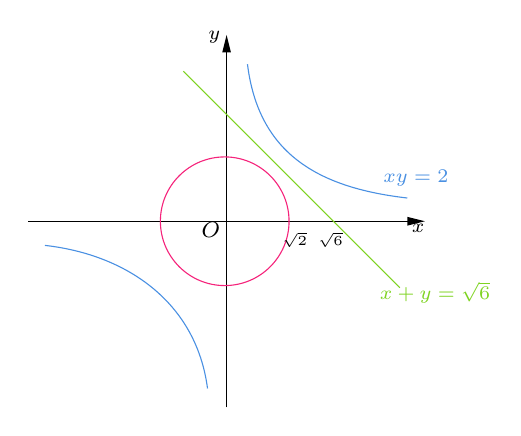
\begin{tikzpicture}[x=0.75pt,y=0.75pt,yscale=-1,xscale=1]
            %uncomment if require: \path (0,300); %set diagram left start at 0, and has height of 300

            %Straight Lines [id:da8026507582116058] 
            \draw    (253,141.76) -- (442.12,141.76) ;
            \draw [shift={(444.12,141.76)}, rotate = 180] [fill={rgb, 255:red, 0; green, 0; blue, 0 }  ][line width=0.08]  [draw opacity=0] (8.4,-2.1) -- (0,0) -- (8.4,2.1) -- cycle    ;
            %Straight Lines [id:da64870239831708] 
            \draw    (348.56,231.5) -- (348.56,54.02) ;
            \draw [shift={(348.56,52.02)}, rotate = 90] [fill={rgb, 255:red, 0; green, 0; blue, 0 }  ][line width=0.08]  [draw opacity=0] (8.4,-2.1) -- (0,0) -- (8.4,2.1) -- cycle    ;
            %Shape: Ellipse [id:dp7551564770874654] 
            \draw  [color={rgb, 255:red, 245; green, 35; blue, 123 }  ,draw opacity=1 ] (316.67,141.76) .. controls (316.67,124.65) and (330.55,110.77) .. (347.66,110.77) .. controls (364.78,110.77) and (378.66,124.65) .. (378.66,141.76) .. controls (378.66,158.88) and (364.78,172.76) .. (347.66,172.76) .. controls (330.55,172.76) and (316.67,158.88) .. (316.67,141.76) -- cycle ;
            %Curve Lines [id:da2129434808692655] 
            \draw [color={rgb, 255:red, 74; green, 144; blue, 226 }  ,draw opacity=1 ]   (358.63,66.12) .. controls (364,109.54) and (393.09,125.65) .. (435.61,130.57) ;
            %Curve Lines [id:da5780763707195247] 
            \draw [color={rgb, 255:red, 74; green, 144; blue, 226 }  ,draw opacity=1 ]   (261.06,153.4) .. controls (300.89,157.88) and (334.01,181.15) .. (339.38,222.33) ;
            %Straight Lines [id:da2981350552987845] 
            \draw [color={rgb, 255:red, 126; green, 211; blue, 33 }  ,draw opacity=1 ]   (327.75,69.48) -- (432.03,173.77) ;

            % Text Node
            \draw (436.55,141.86) node [anchor=north west][inner sep=0.75pt]  [font=\scriptsize]  {$x$};
            % Text Node
            \draw (338.53,48.77) node [anchor=north west][inner sep=0.75pt]  [font=\scriptsize]  {$y$};
            % Text Node
            \draw (335.23,141.09) node [anchor=north west][inner sep=0.75pt]  [font=\footnotesize]  {$O$};
            % Text Node
            \draw (374.19,145.94) node [anchor=north west][inner sep=0.75pt]  [font=\tiny]  {$\sqrt{2}$};
            % Text Node
            \draw (391.4,145.94) node [anchor=north west][inner sep=0.75pt]  [font=\tiny]  {$\sqrt{6}$};
            % Text Node
            \draw (421.19,169.63) node [anchor=north west][inner sep=0.75pt]  [font=\scriptsize,color={rgb, 255:red, 126; green, 211; blue, 33 }  ,opacity=1 ]  {$x+y=\sqrt{6}$};
            % Text Node
            \draw (422.82,115.79) node [anchor=north west][inner sep=0.75pt]  [font=\scriptsize,color={rgb, 255:red, 74; green, 144; blue, 226 }  ,opacity=1 ]  {$xy=2$};


        \end{tikzpicture}
    \end{center}
    根据图象可知, $(x, y)$ 这个点不存在,但其横坐标和纵坐标之和却等于一个实数,两者是存在"矛盾"的。那么问题的关键在哪里?由此从数与形两方面引发学生的认知冲突,让学生面对一种无法弃之不理的"矛盾",从而揭示了引入虚数概念的必要性,虚数的产生变得自然而然。但接下来要解决的问题是如何用几何方式表示复数?
\end{activity}



\subsubsection{新知探究}
1. 复平面

首先,类比实数与数轴上的点一一对应的关系,得到复数与有序实数对对应,而有序实数对又与平面直角坐标系中的点一一对应,所以就可以用平面直角坐标系的点来表示复数。由此介绍复平面、实轴、虚轴等概念。
\begin{itemize}
    \item 实数 $\overset{\text{\tiny 一一对应}}{\longleftrightarrow}$ 数轴上的点
    \item 复数 $\overset{\text{\tiny 一一对应}}{\longleftrightarrow}$ 有序数对 $\overset{\text{\tiny 一一对应}}{\longleftrightarrow}$ 平面直角坐标系上的点
\end{itemize}
\begin{center}

    \tikzset{every picture/.style={line width=0.75pt}} %set default line width to 0.75pt        

    \begin{tikzpicture}[x=0.75pt,y=0.75pt,yscale=-1,xscale=1]
        %uncomment if require: \path (0,300); %set diagram left start at 0, and has height of 300

        %Straight Lines [id:da8790298405518127] 
        \draw    (269,210.55) -- (439.59,210.55) ;
        \draw [shift={(441.59,210.55)}, rotate = 180] [fill={rgb, 255:red, 0; green, 0; blue, 0 }  ][line width=0.08]  [draw opacity=0] (8.4,-2.1) -- (0,0) -- (8.4,2.1) -- cycle    ;
        %Straight Lines [id:da3627886755157933] 
        \draw    (288.92,236.5) -- (288.92,76.42) ;
        \draw [shift={(288.92,74.42)}, rotate = 90] [fill={rgb, 255:red, 0; green, 0; blue, 0 }  ][line width=0.08]  [draw opacity=0] (8.4,-2.1) -- (0,0) -- (8.4,2.1) -- cycle    ;

        %Straight Lines [id:da11661138449086306] 
        \draw [color={rgb, 255:red, 74; green, 144; blue, 226 }  ,draw opacity=1 ] [dash pattern={on 4.5pt off 4.5pt}]  (289.54,120.29) -- (376.24,120.29) ;
        %Straight Lines [id:da8924510381864514] 
        \draw [color={rgb, 255:red, 74; green, 144; blue, 226 }  ,draw opacity=1 ] [dash pattern={on 4.5pt off 4.5pt}]  (376.24,121.58) -- (376.24,210.09) ;
        %Shape: Circle [id:dp8595306873997957] 
        \draw  [fill={rgb, 255:red, 0; green, 0; blue, 0 }  ,fill opacity=1 ] (374.94,120.29) .. controls (374.94,119.57) and (375.52,118.99) .. (376.24,118.99) .. controls (376.96,118.99) and (377.54,119.57) .. (377.54,120.29) .. controls (377.54,121) and (376.96,121.58) .. (376.24,121.58) .. controls (375.52,121.58) and (374.94,121) .. (374.94,120.29) -- cycle ;

        % Text Node
        \draw (275.8,213.46) node [anchor=north west][inner sep=0.75pt]  [font=\footnotesize]  {$O$};
        % Text Node
        \draw (279.28,71.03) node [anchor=north west][inner sep=0.75pt]  [font=\scriptsize]  {$y$};
        % Text Node
        \draw (382.94,102.47) node [anchor=north west][inner sep=0.75pt]    {$Z( a,b)$};
        % Text Node
        \draw (370.69,211.53) node [anchor=north west][inner sep=0.75pt]    {$a$};
        % Text Node
        \draw (274.97,113.76) node [anchor=north west][inner sep=0.75pt]    {$b$};
        % Text Node
        \draw (436.68,213.19) node [anchor=north west][inner sep=0.75pt]  [font=\scriptsize]  {$x$};
        % Text Node
        \draw (422.26,229.22) node [anchor=north west][inner sep=0.75pt]   [align=left] {(实轴)};
        % Text Node
        \draw (232,69.67) node [anchor=north west][inner sep=0.75pt]   [align=left] {(虚轴)};


    \end{tikzpicture}

\end{center}

其中,实轴上的点都表示实数;除了原点外,虚轴上的点都表示纯虚数。

进一步地,因为起点为原点的平面向量与平面直角坐标系中每一个点是一一对应的,所以复数也可以用平面向量来表示。
\begin{center}


    \tikzset{every picture/.style={line width=0.75pt}} %set default line width to 0.75pt        

    \begin{tikzpicture}[x=0.75pt,y=0.75pt,yscale=-1,xscale=1]
        %uncomment if require: \path (0,300); %set diagram left start at 0, and has height of 300

        %Straight Lines [id:da9506260198545818] 
        \draw    (269,210.55) -- (439.59,210.55) ;
        \draw [shift={(441.59,210.55)}, rotate = 180] [fill={rgb, 255:red, 0; green, 0; blue, 0 }  ][line width=0.08]  [draw opacity=0] (8.4,-2.1) -- (0,0) -- (8.4,2.1) -- cycle    ;
        %Straight Lines [id:da10900803625553457] 
        \draw    (288.92,236.5) -- (288.92,76.42) ;
        \draw [shift={(288.92,74.42)}, rotate = 90] [fill={rgb, 255:red, 0; green, 0; blue, 0 }  ][line width=0.08]  [draw opacity=0] (8.4,-2.1) -- (0,0) -- (8.4,2.1) -- cycle    ;

        %Straight Lines [id:da4613502086281518] 
        \draw [color={rgb, 255:red, 74; green, 144; blue, 226 }  ,draw opacity=1 ] [dash pattern={on 4.5pt off 4.5pt}]  (289.54,120.29) -- (376.24,120.29) ;
        %Straight Lines [id:da9023066685141495] 
        \draw [color={rgb, 255:red, 74; green, 144; blue, 226 }  ,draw opacity=1 ] [dash pattern={on 4.5pt off 4.5pt}]  (376.24,121.58) -- (376.24,210.09) ;
        %Shape: Circle [id:dp4067287412354563] 
        \draw  [fill={rgb, 255:red, 0; green, 0; blue, 0 }  ,fill opacity=1 ] (374.94,120.29) .. controls (374.94,119.57) and (375.52,118.99) .. (376.24,118.99) .. controls (376.96,118.99) and (377.54,119.57) .. (377.54,120.29) .. controls (377.54,121) and (376.96,121.58) .. (376.24,121.58) .. controls (375.52,121.58) and (374.94,121) .. (374.94,120.29) -- cycle ;
        %Straight Lines [id:da6206890372549287] 
        \draw [color={rgb, 255:red, 204; green, 26; blue, 137 }  ,draw opacity=1 ][fill={rgb, 255:red, 0; green, 0; blue, 0 }  ,fill opacity=1 ]   (289,210.2) -- (374.85,121.72) ;
        \draw [shift={(376.24,120.29)}, rotate = 134.14] [fill={rgb, 255:red, 204; green, 26; blue, 137 }  ,fill opacity=1 ][line width=0.08]  [draw opacity=0] (12,-3) -- (0,0) -- (12,3) -- cycle    ;

        % Text Node
        \draw (275.8,213.46) node [anchor=north west][inner sep=0.75pt]  [font=\footnotesize]  {$O$};
        % Text Node
        \draw (279.28,71.03) node [anchor=north west][inner sep=0.75pt]  [font=\scriptsize]  {$y$};
        % Text Node
        \draw (382.94,101.47) node [anchor=north west][inner sep=0.75pt]    {$OZ=( a,b)$};
        % Text Node
        \draw (370.69,211.53) node [anchor=north west][inner sep=0.75pt]    {$a$};
        % Text Node
        \draw (274.97,113.76) node [anchor=north west][inner sep=0.75pt]    {$b$};
        % Text Node
        \draw (436.68,213.19) node [anchor=north west][inner sep=0.75pt]  [font=\scriptsize]  {$x$};


    \end{tikzpicture}
\end{center}

这样我们就得到了复数两种等价的几何意义:
\tikzset{every picture/.style={line width=0.75pt}} %set default line width to 0.75pt        
\begin{center}
    \begin{tikzpicture}[x=0.75pt,y=0.75pt,yscale=-1,xscale=1]
        %uncomment if require: \path (0,300); %set diagram left start at 0, and has height of 300


        % Text Node
        \draw (140.99,185.05) node [anchor=north west][inner sep=0.75pt]   [align=left] {复平面上的点$Z( a,b)$};
        % Text Node
        \draw (426.27,187.72) node [anchor=north west][inner sep=0.75pt]   [align=left] {平面向量$\lvec{OZ}=(a,b)$};
        % Text Node
        \draw (327.42,161.12) node [anchor=north west][inner sep=0.75pt]   [align=left] {\textit{一一对应}};
        % Text Node
        \draw (304.67,96.73) node [anchor=north west][inner sep=0.75pt]    {复数$z=a+b\mathrm{i}$};
        % Connection
        \draw    (295.98,198.03) -- (421.27,197.22) ;
        \draw [shift={(423.27,197.21)}, rotate = 179.63] [fill={rgb, 255:red, 0; green, 0; blue, 0 }  ][line width=0.08]  [draw opacity=0] (12,-3) -- (0,0) -- (12,3) -- cycle    ;
        \draw [shift={(293.99,198.04)}, rotate = 359.63] [fill={rgb, 255:red, 0; green, 0; blue, 0 }  ][line width=0.08]  [draw opacity=0] (12,-3) -- (0,0) -- (12,3) -- cycle    ;
        % Connection
        \draw    (338.75,116.33) -- (243.78,179.94) ;
        \draw [shift={(242.12,181.05)}, rotate = 326.19] [color={rgb, 255:red, 0; green, 0; blue, 0 }  ][line width=0.75]    (10.93,-3.29) .. controls (6.95,-1.4) and (3.31,-0.3) .. (0,0) .. controls (3.31,0.3) and (6.95,1.4) .. (10.93,3.29)   ;
        % Connection
        \draw    (375.12,116.33) -- (477.1,182.63) ;
        \draw [shift={(478.77,183.72)}, rotate = 213.03] [color={rgb, 255:red, 0; green, 0; blue, 0 }  ][line width=0.75]    (10.93,-3.29) .. controls (6.95,-1.4) and (3.31,-0.3) .. (0,0) .. controls (3.31,0.3) and (6.95,1.4) .. (10.93,3.29)   ;

    \end{tikzpicture}
\end{center}

2. 复数的模/绝对值

$|z|=|a+b\mathrm{i}|=\sqrt{a^2+b^2}$, 其中 $a, b \in \mathbb{R}$.

3. 共轭复数(参见书本 p71 例 2)

(1) 定义:$z=a+b\mathrm{i}$与$\overline{z}=a-b\mathrm{i}$互为共轭复数。

(2) 几何意义:$z$和$\overline{z}$关于实轴对称。

(3) 性质(看情况补充):
1. $|z|^2=z\overline{z}$;
2. $\overline{z_1+z_2}=\overline{z_1}+\overline{z_2}$;
3. $\overline{z_1 z_2}=\overline{z_1}\cdot\overline{z_2}$;
4. $\overline{\overline{z}}=z$.

\subsubsection{巩固练习}
\begin{example}[改编自书本 p72 例 3]
    设 $z\in \mathbb{C}$,在复平面内对应的点为$Z$,那么满足下列条件的点$Z$的集合是什么图形?
    \begin{enumerate}
        \item $|z|=1$;
        \item $|z|\leqslant 1$;
        \item $|z|< 1$;
        \item $1<|z|\leqslant 2$.
    \end{enumerate}
\end{example}
\begin{solution}
    如图所示,需注意是是圆周还是圆盘,以及边界是否包含在其中。
    \begin{center}


        \tikzset{every picture/.style={line width=0.75pt}} %set default line width to 0.75pt        

        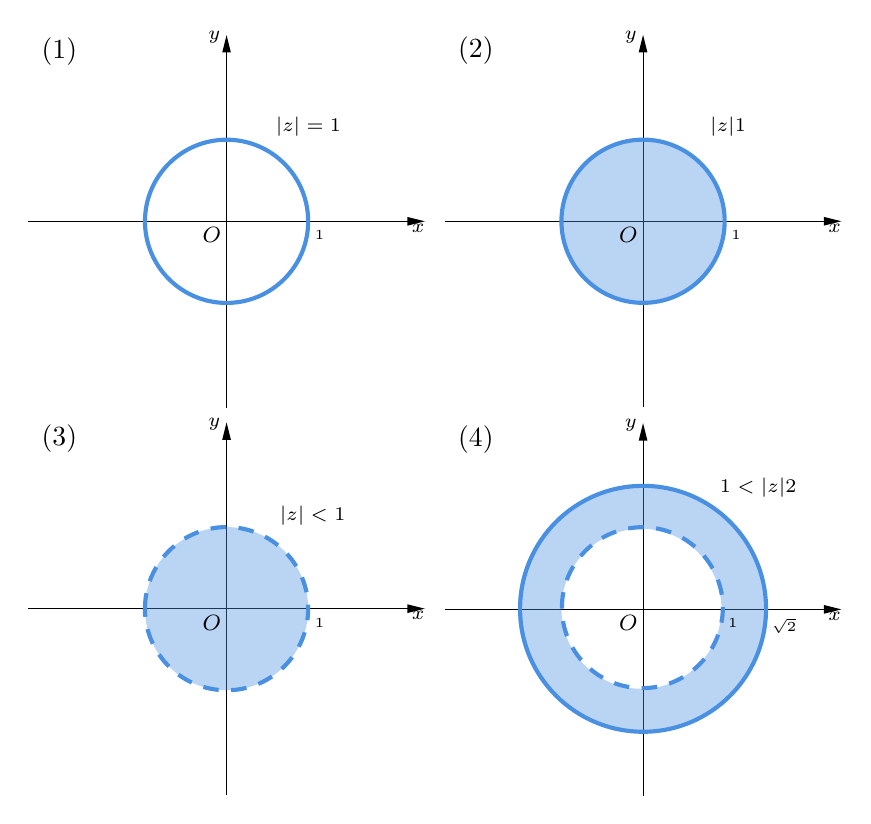
\begin{tikzpicture}[x=0.75pt,y=0.75pt,yscale=-1,xscale=1]
            %uncomment if require: \path (0,498); %set diagram left start at 0, and has height of 498

            %Straight Lines [id:da48952535452117174] 
            \draw    (123.67,111.1) -- (312.78,111.1) ;
            \draw [shift={(314.78,111.1)}, rotate = 180] [fill={rgb, 255:red, 0; green, 0; blue, 0 }  ][line width=0.08]  [draw opacity=0] (8.4,-2.1) -- (0,0) -- (8.4,2.1) -- cycle    ;
            %Straight Lines [id:da7000917064401612] 
            \draw    (219.23,200.84) -- (219.23,23.36) ;
            \draw [shift={(219.23,21.36)}, rotate = 90] [fill={rgb, 255:red, 0; green, 0; blue, 0 }  ][line width=0.08]  [draw opacity=0] (8.4,-2.1) -- (0,0) -- (8.4,2.1) -- cycle    ;
            %Shape: Ellipse [id:dp6427466175006243] 
            \draw  [color={rgb, 255:red, 74; green, 144; blue, 226 }  ,draw opacity=1 ][line width=1.5]  (179.91,111.1) .. controls (179.91,89.38) and (197.51,71.78) .. (219.23,71.78) .. controls (240.94,71.78) and (258.54,89.38) .. (258.54,111.1) .. controls (258.54,132.81) and (240.94,150.42) .. (219.23,150.42) .. controls (197.51,150.42) and (179.91,132.81) .. (179.91,111.1) -- cycle ;
            %Straight Lines [id:da7012394429936882] 
            \draw    (324.33,111.06) -- (513.45,111.06) ;
            \draw [shift={(515.45,111.06)}, rotate = 180] [fill={rgb, 255:red, 0; green, 0; blue, 0 }  ][line width=0.08]  [draw opacity=0] (8.4,-2.1) -- (0,0) -- (8.4,2.1) -- cycle    ;
            %Straight Lines [id:da1521962743776154] 
            \draw    (419.89,200.8) -- (419.89,23.32) ;
            \draw [shift={(419.89,21.32)}, rotate = 90] [fill={rgb, 255:red, 0; green, 0; blue, 0 }  ][line width=0.08]  [draw opacity=0] (8.4,-2.1) -- (0,0) -- (8.4,2.1) -- cycle    ;
            %Shape: Ellipse [id:dp8009519989013992] 
            \draw  [color={rgb, 255:red, 74; green, 144; blue, 226 }  ,draw opacity=1 ][fill={rgb, 255:red, 74; green, 144; blue, 226 }  ,fill opacity=0.38 ][line width=1.5]  (380.57,111.06) .. controls (380.57,89.35) and (398.18,71.75) .. (419.89,71.75) .. controls (441.61,71.75) and (459.21,89.35) .. (459.21,111.06) .. controls (459.21,132.78) and (441.61,150.38) .. (419.89,150.38) .. controls (398.18,150.38) and (380.57,132.78) .. (380.57,111.06) -- cycle ;
            %Straight Lines [id:da04562857260938191] 
            \draw    (123.67,297.73) -- (312.78,297.73) ;
            \draw [shift={(314.78,297.73)}, rotate = 180] [fill={rgb, 255:red, 0; green, 0; blue, 0 }  ][line width=0.08]  [draw opacity=0] (8.4,-2.1) -- (0,0) -- (8.4,2.1) -- cycle    ;
            %Straight Lines [id:da12411551232842866] 
            \draw    (219.23,387.47) -- (219.23,209.99) ;
            \draw [shift={(219.23,207.99)}, rotate = 90] [fill={rgb, 255:red, 0; green, 0; blue, 0 }  ][line width=0.08]  [draw opacity=0] (8.4,-2.1) -- (0,0) -- (8.4,2.1) -- cycle    ;
            %Shape: Ellipse [id:dp9648039203988316] 
            \draw  [color={rgb, 255:red, 74; green, 144; blue, 226 }  ,draw opacity=1 ][fill={rgb, 255:red, 74; green, 144; blue, 226 }  ,fill opacity=0.38 ][dash pattern={on 5.63pt off 4.5pt}][line width=1.5]  (179.91,297.73) .. controls (179.91,276.02) and (197.51,258.41) .. (219.23,258.41) .. controls (240.94,258.41) and (258.54,276.02) .. (258.54,297.73) .. controls (258.54,319.45) and (240.94,337.05) .. (219.23,337.05) .. controls (197.51,337.05) and (179.91,319.45) .. (179.91,297.73) -- cycle ;
            %Straight Lines [id:da5391729869714962] 
            \draw    (324.33,298.06) -- (513.45,298.06) ;
            \draw [shift={(515.45,298.06)}, rotate = 180] [fill={rgb, 255:red, 0; green, 0; blue, 0 }  ][line width=0.08]  [draw opacity=0] (8.4,-2.1) -- (0,0) -- (8.4,2.1) -- cycle    ;
            %Straight Lines [id:da2784087258564013] 
            \draw    (419.89,387.8) -- (419.89,210.32) ;
            \draw [shift={(419.89,208.32)}, rotate = 90] [fill={rgb, 255:red, 0; green, 0; blue, 0 }  ][line width=0.08]  [draw opacity=0] (8.4,-2.1) -- (0,0) -- (8.4,2.1) -- cycle    ;
            %Shape: Donut [id:dp063216757672522] 
            \draw  [color={rgb, 255:red, 0; green, 0; blue, 0 }  ,draw opacity=0 ][fill={rgb, 255:red, 74; green, 144; blue, 226 }  ,fill opacity=0.38 ,even odd rule] (380.57,297.79) .. controls (380.57,276.5) and (397.83,259.25) .. (419.11,259.25) .. controls (440.4,259.25) and (457.65,276.5) .. (457.65,297.79) .. controls (457.65,319.07) and (440.4,336.32) .. (419.11,336.32) .. controls (397.83,336.32) and (380.57,319.07) .. (380.57,297.79)(359.59,297.79) .. controls (359.59,264.91) and (386.24,238.26) .. (419.11,238.26) .. controls (451.99,238.26) and (478.63,264.91) .. (478.63,297.79) .. controls (478.63,330.66) and (451.99,357.31) .. (419.11,357.31) .. controls (386.24,357.31) and (359.59,330.66) .. (359.59,297.79) ;
            %Shape: Ellipse [id:dp07345428958267963] 
            \draw  [color={rgb, 255:red, 74; green, 144; blue, 226 }  ,draw opacity=1 ][line width=1.5]  (360.65,297.79) .. controls (360.65,265.07) and (387.17,238.54) .. (419.89,238.54) .. controls (452.61,238.54) and (479.14,265.07) .. (479.14,297.79) .. controls (479.14,330.51) and (452.61,357.03) .. (419.89,357.03) .. controls (387.17,357.03) and (360.65,330.51) .. (360.65,297.79) -- cycle ;
            %Shape: Ellipse [id:dp08448019654683137] 
            \draw  [color={rgb, 255:red, 74; green, 144; blue, 226 }  ,draw opacity=1 ][fill={rgb, 255:red, 255; green, 255; blue, 255 }  ,fill opacity=0 ][dash pattern={on 5.63pt off 4.5pt}][line width=1.5]  (380.79,297.24) .. controls (380.79,275.83) and (398.15,258.47) .. (419.56,258.47) .. controls (440.98,258.47) and (458.33,275.83) .. (458.33,297.24) .. controls (458.33,318.65) and (440.98,336.01) .. (419.56,336.01) .. controls (398.15,336.01) and (380.79,318.65) .. (380.79,297.24) -- cycle ;

            % Text Node
            \draw (507.88,111.16) node [anchor=north west][inner sep=0.75pt]  [font=\scriptsize]  {$x$};
            % Text Node
            \draw (409.86,18.07) node [anchor=north west][inner sep=0.75pt]  [font=\scriptsize]  {$y$};
            % Text Node
            \draw (407.07,112.89) node [anchor=north west][inner sep=0.75pt]  [font=\footnotesize]  {$O$};
            % Text Node
            \draw (461.21,114.46) node [anchor=north west][inner sep=0.75pt]  [font=\tiny]  {$1$};
            % Text Node
            \draw (329.56,21.14) node [anchor=north west][inner sep=0.75pt]   [align=left] {(2)};
            % Text Node
            \draw (241.67,59.73) node [anchor=north west][inner sep=0.75pt]  [font=\scriptsize]  {$| z| =1$};
            % Text Node
            \draw (451,59.73) node [anchor=north west][inner sep=0.75pt]  [font=\scriptsize]  {$| z| \leqslant 1$};
            % Text Node
            \draw (243.67,247.07) node [anchor=north west][inner sep=0.75pt]  [font=\scriptsize]  {$| z| < 1$};
            % Text Node
            \draw (455.67,233.73) node [anchor=north west][inner sep=0.75pt]  [font=\scriptsize]  {$1< | z| \leqslant 2$};
            % Text Node
            \draw (307.22,297.83) node [anchor=north west][inner sep=0.75pt]  [font=\scriptsize]  {$x$};
            % Text Node
            \draw (209.2,204.73) node [anchor=north west][inner sep=0.75pt]  [font=\scriptsize]  {$y$};
            % Text Node
            \draw (206.4,299.55) node [anchor=north west][inner sep=0.75pt]  [font=\footnotesize]  {$O$};
            % Text Node
            \draw (260.54,301.13) node [anchor=north west][inner sep=0.75pt]  [font=\tiny]  {$1$};
            % Text Node
            \draw (128.89,207.8) node [anchor=north west][inner sep=0.75pt]   [align=left] {(3)};
            % Text Node
            \draw (507.88,298.16) node [anchor=north west][inner sep=0.75pt]  [font=\scriptsize]  {$x$};
            % Text Node
            \draw (409.86,205.07) node [anchor=north west][inner sep=0.75pt]  [font=\scriptsize]  {$y$};
            % Text Node
            \draw (407.07,299.89) node [anchor=north west][inner sep=0.75pt]  [font=\footnotesize]  {$O$};
            % Text Node
            \draw (459.65,301.19) node [anchor=north west][inner sep=0.75pt]  [font=\tiny]  {$1$};
            % Text Node
            \draw (329.56,208.14) node [anchor=north west][inner sep=0.75pt]   [align=left] {(4)};
            % Text Node
            \draw (307.22,111.2) node [anchor=north west][inner sep=0.75pt]  [font=\scriptsize]  {$x$};
            % Text Node
            \draw (209.2,18.1) node [anchor=north west][inner sep=0.75pt]  [font=\scriptsize]  {$y$};
            % Text Node
            \draw (206.4,112.92) node [anchor=north west][inner sep=0.75pt]  [font=\footnotesize]  {$O$};
            % Text Node
            \draw (260.54,114.5) node [anchor=north west][inner sep=0.75pt]  [font=\tiny]  {$1$};
            % Text Node
            \draw (128.89,21.17) node [anchor=north west][inner sep=0.75pt]   [align=left] {(1)};
            % Text Node
            \draw (480.63,301.19) node [anchor=north west][inner sep=0.75pt]  [font=\tiny]  {$\sqrt{2}$};


        \end{tikzpicture}

    \end{center}
\end{solution}

\subsubsection{小结}
虚数 (imaginary) 这个名称是法国哲学家、数学家笛卡儿给出的,写在 1637 年出版的《几何》中。欧拉第一个使用符号$\mathrm{i}$表示虚数,写在 1777 年提交给圣彼得堡科学院的论文中,这篇论文直到 1794 年才发表。

只有给出复数的几何表示,人们才真正感觉到了复数的存在,才心安理得地接受了复数。

1797 年,丹麦测量学家韦塞尔在丹麦皇家科学院宣读了一篇关于复数的论文,文中引入了虚轴、并把复数表示为平面向量。但直到 100 年后的 1897 年,韦塞尔的丹麦文的论文被翻译为法文后,复数几何表示的工作才引起数学界的广泛重视。

瑞士数学家阿尔冈把复数对应的向量的长度称为模,写在 1806 年出版的著作《试论几何作图中虚量的表示法》中,他还进一步利用三角函数表示复数。

现在,复数已经被广泛应用于流体力学、信号分析等学科,因此复数有着深厚的物理背景。在复数的基础上,英国数学家哈密顿构造了四元数,并导致了物理学中著名的麦克斯韦方程的产生。

在数学史上,虚数以及复数概念的引入经历了一个曲折的过程,其中充满着数学家的想象力、创造力和不屈不挠、精益求精的精神,时至今日仍然值得我们学习和借鉴!






%\input{data/chap08_立体几何初步.tex}

\bibliography{refs} % 设置参考文献文件为references.bib
\end{document}